\begin{filecontents}{apsrevcontrol.bib}
  @CONTROL{apsrev41Control,title="0"%,author="48",editor="1",pages="1",year="0"}
\end{filecontents}
\RequirePackage[l2tabu, orthodox]{nag}
\documentclass[aps,english,superscriptaddress,twocolumn,twoside,longbibliography,prl,floatfix]{revtex4-1}%

\usepackage[utf8]{inputenx}% for arXiv use encoding ansinew
%\input{ix-utf8enc.dfu}
\usepackage[OT1]{fontenc}
\usepackage{amsfonts}
\usepackage{amssymb}
\usepackage{amsthm}
\usepackage{amsmath}
\usepackage{graphicx}%
\setcounter{MaxMatrixCols}{30}
%TCIDATA{OutputFilter=latex2.dll}
%TCIDATA{Version=5.50.0.2953}
%TCIDATA{CSTFile=revtex4.cst}
%TCIDATA{Created=Thursday, February 14, 2013 01:09:34}
%TCIDATA{LastRevised=Thursday, February 21, 2013 15:16:22}
%TCIDATA{<META NAME="GraphicsSave" CONTENT="32">}
%TCIDATA{<META NAME="SaveForMode" CONTENT="1">}
%TCIDATA{BibliographyScheme=Manual}
%TCIDATA{<META NAME="DocumentShell" CONTENT="Articles\SW\REVTeX 4">}
%BeginMSIPreambleData
\providecommand{\U}[1]{\protect\rule{.1in}{.1in}}
%EndMSIPreambleData
\newtheorem{theorem}{Theorem}
\newtheorem{acknowledgement}[theorem]{Acknowledgement}
\newtheorem{algorithm}[theorem]{Algorithm}
\newtheorem{axiom}[theorem]{Axiom}
\newtheorem{claim}[theorem]{Claim}
\newtheorem{conclusion}[theorem]{Conclusion}
\newtheorem{condition}[theorem]{Condition}
\newtheorem{conjecture}[theorem]{Conjecture}
\newtheorem{corollary}[theorem]{Corollary}
\newtheorem{criterion}[theorem]{Criterion}
\newtheorem{definition}[theorem]{Definition}
\newtheorem{example}[theorem]{Example}
\newtheorem{exercise}[theorem]{Exercise}
\newtheorem{lemma}[theorem]{Lemma}
\newtheorem{notation}[theorem]{Notation}
\newtheorem{problem}[theorem]{Problem}
\newtheorem{proposition}[theorem]{Proposition}
\newtheorem{remark}[theorem]{Remark}
\newtheorem{solution}[theorem]{Solution}
\newtheorem{summary}[theorem]{Summary}
%\newenvironment{proof}[1][Proof]{\noindent\textbf{#1.} }{\ \rule{0.5em}{0.5em}}

% hyperlink stuff
\usepackage[usenames,dvipsnames]{color}
\definecolor{ultramarine}{RGB}{63, 0, 255}
\definecolor{medblue}{RGB}{0, 0, 100}
\definecolor{panblue}{RGB}{0,24,150}
\definecolor{carmine}{RGB}{150, 0, 24}
\usepackage[breaklinks=true]{hyperref}
\hypersetup{colorlinks,
linkcolor=carmine,
citecolor=medblue,
urlcolor=panblue,
anchorcolor=OliveGreen}
%\usepackage{url}


\definecolor{purple}{RGB}{128,0,128}
\newcommand{\purp}[1]{{\color{purple}{#1}\color{black}}}

\usepackage{verbatim} %for comment command
\usepackage{units}% for nicefrac
\newcommand{\half}[1]{\nicefrac{#1}{2}}

\usepackage{braket} %provide \bra and \Bra and \set and \Set etc...
\newcommand{\brackets}[1]{\lbrace{#1\rbrace}}
%\newcommand{\brackets}{\Set}



\usepackage{microtype}
\usepackage[capitalise]{cleveref}
\Crefname{eqs}{Eqs.}{Eqs.}
\creflabelformat{eqs}{(#2#1#3)}
\crefrangelabelformat{equation}{(#3#1#4-#5#2#6)}
%\crefmultiformat{equation}{eqs.~(#2#1#3)}{ and~(#2#1#3)}{, (#2#1#3)}{ and~(#2#1#3)}
\Crefmultiformat{equation}{Eqs.~(#2#1#3}{,#2#1#3)}{,#2#1#3}{,#2#1#3)}

\usepackage{mathtools} %for mathclap and prescript and more. Learning to love this package. And DeclarePairDelimeter!
\DeclarePairedDelimiter\ceil{\lceil}{\rceil}
\DeclarePairedDelimiter\floor{\lfloor}{\rfloor}
\DeclarePairedDelimiter\parens{\lparen}{\rparen}

%\usepackage{nath} %automatically pair delimiters. Provides \inline and \displayed. Adjusts \frac and /

\newcommand{\naf}{\ensuremath{\mathring{a}}}
\newcommand{\nbf}{\ensuremath{\mathring{b}}}
\newcommand{\ncf}{\ensuremath{\mathring{c}}}

\newcommand{\na}{\ensuremath{\lnot a}}
\newcommand{\nb}{\ensuremath{\lnot b}}
\newcommand{\nc}{\ensuremath{\lnot c}}


\newcommand{\nap}{\ensuremath{a^{\prime}}}
\newcommand{\nbp}{\ensuremath{b^{\prime}}}
\newcommand{\ncp}{\ensuremath{c^{\prime}}}

\newcommand{\p}[1]{\ensuremath{p\parens{#1}}}
\newcommand{\cramp}[1]{\ensuremath{\mathord{#1}}}
\newcommand{\eql}{\cramp{=}}

%\newcommand{\cramp}[1]{\ensuremath{\mathopen{}#1\mathclose{}}}



\begin{document}
%\preprint{ }
%\title{Transitivity of implication and causal structure}
\title{Alternatives to Entropic Inequalities and the Triangle Scenario}
\author{Robert W. Spekkens}
\email{rspekkens@perimeterinstitute.ca}
\affiliation{Perimeter Institute for Theoretical Physics, Waterloo, Ontario, Canada, N2L 2Y5}
\author{Tobias Fritz}
\email{tfritz@perimeterinstitute.ca}
\affiliation{Perimeter Institute for Theoretical Physics, Waterloo, Ontario, Canada, N2L 2Y5}
\author{Elie Wolfe}
\email{ewolfe@perimeterinstitute.ca}
\affiliation{Perimeter Institute for Theoretical Physics, Waterloo, Ontario, Canada, N2L 2Y5}
\date{\today}


\begin{abstract}
Given some hypothesis of causal structure it is desirable to determine the set of probability distributions compatible with the hypothesis. For certain causal structures, such as Bell scenarios, the compatible set corresponds to the convex hull of various deterministic distributions, and admits a necessary and sufficient description in terms of conditional probability linear inequalities. For more general causal structures, however, it is far easier to derive entropic inequalities instead of probabilistic inequalities. Unfortunately there typically exist distributions which are genuinely incompatible with the causal structure but which satisfy all the structure's entropic inequalities. A tight characterization of all distributions which can be explained in terms of classical latent variables is critical in quantum information theory in order to recognize and exploit uniquely quantum distributions. The insufficiency of entropic inequalities, therefore, motivates us to explore alternative means of deriving compatibility tests for general causal structures, ideally directly at the level of probabilities. Uniquely quantum distributions are known to exist in the Triangle scenario; the methods presented herein may assist in isolating the criteria which distinguish quantum from classical distributions in that scenario.
\end{abstract}
\maketitle
%In Ref.~\cite{WoodSpekkens}, the standard proof of Bell's theorem is presented in the language of causal inference.  In particular, the CHSH inequality emerges as a special case of what Pearl calls an ``instrumental inequality''.  Hardy's proof of Bell's theorem is quite different from the standard proof and the following question naturally arises: is there a generic tool for classical causal inference of which the Hardy argument can be considered a special case when applied to the M-shaped causal structure of the Bell experiment?

%To try and answer this question, we apply Hardy-type reasoning to the triangle causal structure, that is, the one with three observed variables, each pair of which have a common cause.  We show that this sort of reasoning does indeed facilitate causal inference in the case of the triangle causal structure, thereby lending some evidence to the notion that this style of argument has the potential to be generalized into a generic tool for classical causal inference.

\section{Introduction}
***needs introduction***

\section{Transitive Inference Paradoxes}

Per Ref.~[\citealp[]{LSW}, see also \citealp[]{H.Stapp:Hardy:Transitivity,D.Boschi:PRL:2755,Mermin,Unruh}], the Hardy-type proof of nonlocality~\cite{L.Hardy:PRL:1665} is fundamentally an expression of the the transitivity of implications among value assignments in noncontextual ontological models. Transitivity follows from noncontextuality because value assignments do not depend on the context (local or remote) of the measurement. Failure of the transitivity of implication therefore implies the impossibility of such models. We begin by recalling the Hardy paradox in this form, and then show how the assumption of transitivity can be replaced with the assumption of a particular causal structure. 

We follow the convention that upper-case indicates random variables while lower-case indicates some value associated with the random variable. Thus $p(ab|xy\lambda)$ should be understood as ${p(A\mathopen{=}a,B\mathopen{=}b|X\mathopen{=}x,Y\mathopen{=}y,\Lambda\mathopen{=}\lambda)}$. We use lower-case subscripts to indicate conditioning upon a particular value, such that for instance $p(a_x b_y|\lambda)=p(ab|xy\lambda)$. We also take $\nb$ to mean ``anything but $b$", and accordingly $P(\na,\nb)=P(A\mathopen{\neq}a,B\mathopen{\neq}b)$.

Suppose that Alice and Bob can each make simultaneous inquiries of various binary observables, but subject to the restriction that each party can only examine one of his or her local observables in a given trial. Let Alice's (Bob's) observables be $\brackets{A_0,A_1}$ ($\brackets{B_0,B_1}$).

Now, suppose after performing many trials Alice and Bob are confident in the measurement statistics that three events never occur:
\begin{align}\begin{split}\label{eq:hardydisjunctive}
\text{never }& \left[a_0,\nb_1\right],
\; \text{never } \left[\na_1,b_0\right],
\; \text{never } \left[a_1, b_1\right].
\end{split}\end{align}
For the purpose of discussion possible implication of these statistics it is convenient to re-express \cref{eq:hardydisjunctive} in an equivalent but contrapositive form, namely 
\begin{align}\begin{split}\label{eq:hardycontrapositive}
a_0 &\implies b_1,
\; b_0 \implies a_1,
\; b_1 \implies \na_1.
\end{split}\end{align}
Now, if transitivity were to hold in \cref{eq:hardycontrapositive} then one could infer that 
\begin{align}\label{eq:hardyimplication}
a_0 &\implies b_1 \implies \na_1 \implies \nb_0
\end{align}
where the last implication was via modus tollens. The overall implication is equivalent to
\begin{align}\label{eq:hardyimplied}
\text{ never }\left[a_0,b_0\right].
\end{align}
%or back to disjunctive form, \cref{eq:hardydisjunctive} plus transitivity implies
%\begin{align}\label{eq:hardyimplicationdisjunctive}
%\text{never}&\quad \left[A_0,B_1\right].
%\end{align}
Thus this proof shows that the distribution known as the PR box~\cite{PROriginal,PRUnit}
\begin{align}\label{eq:PRbox}
p_{\text{PR}}(a_x b_y)=\begin{cases}\nicefrac{1}{2}&\text{if }\; a\oplus b= x y \\ 0&\text{otherwise}\end{cases},
\end{align}
where $a,b,x,y\in\brackets{0,1}$,
is incompatible with noncontextual ontological models, because it satisfies \cref{eq:hardydisjunctive} but not \cref{eq:hardyimplied}. 
%Note that in \cref{eq:PRbox} we have employed the shorthand 
%\begin{align}\label{eq:allbutone}
%a^{\prime}=\begin{cases} 1 &\text{if }a=1 \\ 0 & \text{if }a\neq 1\end{cases}
%\end{align}
%etc.

\section{Hardy Criteria Via Causal Inference}

It is often claimed that classically one must have $p\left(a_1 b_1\right)\geq p\left(a_0 b_0\right)$ from just the first two conditions in  \cref{eq:hardycontrapositive} alone \cite{CabelloHardyInequality}, such that the result ``If additionally $p\left(a_1 b_1\right)=0$ then $p\left(a_0 b_0\right)=0$" is just a special case. We now demonstrate that this Hardy-type inequality follows naturally from assumptions about causal structure. More importantly, we show that Hardy-type arguments can be used to derive compatibility criteria in the same vein even for general causal structures.

\begin{figure}[t!]
 \center{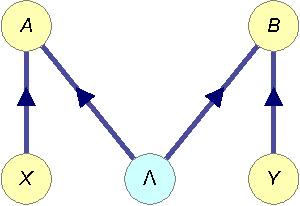
\includegraphics[width=2in]{BellDAGcap.pdf}}
\caption{The causal structure of the Bell scenario, on which Bell's theorem is based.}
 \label{fig:BellDAG}
\end{figure}

Consider the causal structure associated to the Bell experiment, depicted in \cref{fig:BellDAG}. $\brackets{A,B,X,Y}$ are all observable variables whereas $\lambda$ is the latent common cause of $A$ and $B$.

%Without loss of generality let's assume that the values $\Lambda\mathopen{=}\lambda$ are drawn from some (possibly infinite, possibly continuous) set $\lambda\in\Omega$. 
The assumption of causal structure dictates that
\begin{align}\begin{split}\label{eq:bellstructure}
p&\parens{a,b|x,y,\lambda}=p\left(a_x|\lambda\right)p\left(b_y|\lambda\right)
\end{split}\end{align}
and accordingly that
\begin{align}\begin{split}\label{eq:bellintegration}
&p\left(ab|xy\right)
=\int\limits_{\mathclap{\text{all }\lambda}}p\left(a_x|\lambda\right)p\left(b_y|\lambda\right)p\left(\lambda\right).
\end{split}\end{align}


Now, the contrapositive conditions in \cref{eq:hardycontrapositive} can be rephrased in terms of $\Lambda$, in the sense that, say, any $\lambda$ which gives rise to $a_0$ must -- with probability 1 -- also give rise to $b_1$. Formally, ``$a_0$ implies $b_1$" is equivalent to ``$\forall_\lambda\!:\;\text{if }p\left(a_0|\lambda\right)\neq 0 \text{ then }p\left(b_1|\lambda\right)=1$". This inequality, together with the causal structure implication of \cref{eq:bellintegration}, leads to


%We can also define (possibly empty) subsets of $\Omega$ which consists of those $\lambda$ for which certain functional dependencies are guaranteed, such as 
%\begin{align}
%\Omega{\left[a_x,b_y\right]} \;:\; \forall_{\lambda \in \Omega_{\left[a_x,b_y\right]}} p\left(a_x b_y|\lambda\right)\neq 0.
%\end{align}
%\begin{align}\label{eq:def:omegastar}
%\Omega_* \;:\; \forall_{\lambda \in \Omega_*} p\left(\left[A_x,B_y\right]||\lambda\right)>0.
%\end{align}
%Note that the exists statement such as $\exists_{\lambda_*} {\lambda_* \in \Omega_*}$ are equivalent to  $\int_{\lambda \in \Omega_*} p\left(\lambda\right)>0$.

\begin{proposition} \label{prop:BellNoGo}
The Bell causal structure (\cref{fig:BellDAG}) implies
\begin{align}
{\rm if  }\;\; &p\left(a_0 b_1\right)=p\left(a_9\right),\label{eq:A0impB1source}\\
{\rm and }\;\; &p\left(a_1 b_0\right)=p\left(b_0\right),\label{eq:B0impA1source}\\
{\rm then }\;\; &p\left(a_0 b_0\right)\leq p\left(a_1 b_1\right) .\label{eq:cabelloresult}
\end{align}
\end{proposition}

\begin{proof}
Note that \cref{eq:A0impB1source,eq:B0impA1source} are identical to the first two conditions in \cref{eq:hardycontrapositive}. In terms of the latent variables the contrapositive statements imply
\begin{align}
&\forall_{\lambda}\; %=
p\left(b_1|\lambda\right)\geq p\left(a_0|\lambda\right) ,\label{eq:A0eqB1}
\\&\forall_{\lambda}\; 
p\left(b_0|\lambda\right)\geq p\left(a_1|\lambda\right).\label{eq:B0eqA1}
%\\&\exists_{\lambda_*} {\lambda_* \in \Omega_*}
%\exists_{\lambda_*}\; p\left(\lambda_*\right)>0,\;p\left(\left[A_0\right]||\lambda_*\right)>0,\;p\left(\left[B_0\right]||\lambda_*\right)>0
%,\label{eq:A0B0pos}
\end{align}
Substitution into \cref{eq:bellintegration} then implies
\begin{align}\begin{split}\label{eq:hardyintegrals}
p\left(a_0 b_0\right)&=\int_\lambda%\limits_{\mathclap{\text{all }\lambda}}
p\left(a_0|\lambda\right)p\left(b_0|\lambda\right)p\left(\lambda\right)\\
%&=\int\limits_{\mathclap{\lambda\in \Omega{\left[a_0 b_0\right]}}} p\left(a_0|\lambda\right)p\left(b_0|\lambda\right)p\left(\lambda\right)\\
&\leq \int_\lambda%\limits_{\mathclap{\text{all }\lambda}}
p\left(b_1|\lambda\right)p\left(a_1|\lambda\right)p\left(\lambda\right)\\
%&\leq\int\limits_{\mathclap{\lambda\in \Omega}} p\left(b_1|\lambda\right)p\left(a_1|\lambda\right)p\left(\lambda\right)\\
&=p\left(a_1 b_1\right)\qedhere
\end{split}\end{align}
%The idea which converts this argument into something practical, i.e. upgrades \cref{eq:hardyintegrals} into Prop.~\ref{prop:BellNoGo}, is that deterministic relationships between observed variables are equivalent to For-All statements regarding their common causes under the assumption of causal structure.
%
%In our example, \cref{eq:A0eqB1,eq:B0eqA1} are derivable from the observable statistics posited in \cref{eq:A0impB1source,eq:B0impA1source} respectively. \cref{eq:A0eqB1,eq:B0eqA1} follow from \cref{eq:A0impB1source,eq:B0impA1source} because any $\lambda$ which even occasionally gives rise to $a_0$ must also certainly give rise to $b_1$ as the observable statistics prohibit the events $\left[a_0,\nb_1\right]$ or $\left[\na_1,B_0\right]$.
%To be clear, if $p\left(a_0|\lambda\right)=0$ then the \cref{eq:A0impB1source} is thoroughly uninformative regarding $p\left(b_1|\lambda\right)$, as any such $\lambda$ is excluded from consideration in \cref{eq:A0eqB1}.
\end{proof}

\section{The triangle causal structure}

The same causal inference logic can be applied to the Triangle scenario, namely the causal structure depicted in \cref{fig:TriDAG}. Here $\brackets{A,B,C}$ and the observed variables, and  $\brackets{\Lambda_{AB},\Lambda_{BC},\Lambda_{AC}}$ are latent. $\Lambda_{AB}$ denotes the common cause of $A$ and $B$, etc. 


\begin{figure}[!t]
 \center{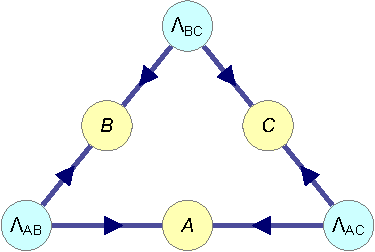
\includegraphics[width=2.5in]{TriDAGcap.pdf}}
\caption{The causal structure of the Triangle scenario, for which the three observed variables lack a common ancestor.}
 \label{fig:TriDAG}
\end{figure}


The Triangle scenario's causal structure dictates that
\begin{align}\begin{split}\label{eq:tristructure}
p&(abc|\lambda_{AB}\lambda_{BC}\lambda_{AC})\\
&=p(a\lambda_{AB}\lambda_{AC})p(b\lambda_{AB}\lambda_{BC})p(c|\lambda_{BC}\lambda_{AC}).
\end{split}\end{align}
%For excessive clarity, let $\Omega_{AB}\left[\_\_\right]$ denote the complete set of values which $\lambda_{AB}$ can take, and let $\Omega_{AB}\left[a\_\right]$ denote the special subset of possible $\lambda_{AB}$ for which ${P\left(a|\lambda_{AB}\right)\neq 0}$. %$\exists_{\lambda_{AC}}\!:\; {P\left(a|\lambda_{AB}\lambda_{AC}\right)>0}$.
Accordingly,
\begin{align}\label{eq:triintegration}
&p(abc)=\\\nonumber
&\int\!\!\int\limits_{\mathclap{\lambda_{AB}\lambda_{BC}\lambda_{AC}}}\!\!\int
%\limits_{\mathclap{\substack{\lambda_{AB}\in \Omega_{AB}\left[\_\_\right]\\\lambda_{BC}\in \Omega_{BC}\left[\_\_\right]\\\lambda_{AC}\in \Omega_{AC}\left[\_\_\right]}}}
\begin{pmatrix}p(a|\lambda_{AB}\lambda_{AC})p(b|\lambda_{AB}\lambda_{BC})p(c|\lambda_{BC}\lambda_{AC})\\
\times p(\lambda_{AB})p(\lambda_{BC})p(\lambda_{AC})\end{pmatrix}
\end{align}

%\begin{align}\label{eq:triintegration}
%p&\left(A\mathopen{=}a,B\mathopen{=}b,C\mathopen{=}c\right)
%\\\nonumber&=\int\limits_{\mathclap{\substack{\lambda_{AB}\in \Omega_{AB}\\\lambda_{BC}\in \Omega_{BC}\\\lambda_{AC}\in \Omega_{AC}}}}\!\!\begin{pmatrix}p\left(A\mathopen{=}a|\lambda_{AB},\lambda_{AC}\right) p\left(B\mathopen{=}b|\lambda_{AB},\lambda_{BC}\right)\times\\ p\left(C\mathopen{=}c|\lambda_{AC},\lambda_{BC}\right)p\left(\lambda_{AB}\right)p\left(\lambda_{BC}\right) p\left(\lambda_{AC}\right)\end{pmatrix}.
%\end{align}

\begin{proposition} \label{prop:TriNoGo}
The Triangle causal structure (\cref{fig:TriDAG}) implies that, for any $\brackets{\nap,\nbp,\ncp}$,
\begin{align}
{\rm if  }\;\; &p\left(a\nbp\right)=p\left(a\right),\label{eq:AimpNotBsource}\\
{\rm and }\;\; &p\left(b\ncp\right)=p\left(b\right),\label{eq:BimpNotCsource}\\
{\rm and }\;\; &p\left(\nap c\right)=p\left(c\right),\label{eq:CimpNotAsource}\\
{\rm then }\;\; &p\left(a\right)p\left(b\right)p\left(c\right)\leq p\left(\nap\nbp\ncp\right).\label{eq:spekkensresult}
\end{align}
As $p\left(abc\right)\geq p\left(a\right)p\left(b\right)p\left(c\right)$ for any causal structure, the proposition is strongest when $\nap=\na$ etc.
\end{proposition}

\begin{proof}
First we convert the deterministic relations supposed by \cref{eq:AimpNotBsource,eq:BimpNotCsource,eq:CimpNotAsource} into contrapositive statements; they state that $a\implies \nbp$, $b\implies\ncp$, and $c\implies\nap$. Now, if $X\mathopen{=}x\implies Y\mathopen{=}y$ then whenever the common latent parent of $X$ and $Y$ takes on a value which give rise to $X\cramp{=}x$ we can be assured that $Y$ also takes on the value of $y$ regardless of values of any other of $Y$'s parent variables. As such, \cref{eq:AimpNotBsource,eq:BimpNotCsource,eq:CimpNotAsource} further imply that
\begin{align}
&\forall_{\lambda_{AB} }\; p\left(\nb|\lambda_{AB},\lambda_{BC}\right)\geq p\left(a|\lambda_{AB}\right)\\
&\forall_{\lambda_{BC} }\; p\left(\nc|\lambda_{BC},\lambda_{AC}\right)\geq p\left(b|\lambda_{BC}\right)\\
&\forall_{\lambda_{AC} }\; p\left(\na|\lambda_{AC},\lambda_{AB}\right)\geq p\left(c|\lambda_{AC}\right)
\end{align}
It then follows that
\begin{align}
\nonumber p&\left(a\right)p\left(b\right)p\left(c\right)
%\\\nonumber &=\!\int\limits_{\mathclap{\lambda_{AB},\lambda_{BC},\lambda_{AC}}}
%\\\nonumber &=\!\int\limits_{\lambda_{AB}}\!\int\limits_{\lambda_{BC}}\!\int\limits_{\lambda_{AC}}
\\ &=\!\int\!\!\int\limits_{\mathclap{\lambda_{AB}\lambda_{BC}\lambda_{AC}}}\!\!\int
%\limits_{\mathclap{\substack{\lambda_{AB}\in \Omega_{AB}\left[\_\_\right]\\\lambda_{BC}\in \Omega_{BC}\left[\_\_\right]\\\lambda_{AC}\in \Omega_{AC}\left[\_\_\right]}}}
\begin{pmatrix}p\left(a|\lambda_{AB}\right) p\left(b|\lambda_{BC}\right)p\left(c|\lambda_{AC}\right)\times\\ p\left(\lambda_{AB}\right)p\left(\lambda_{BC}\right) p\left(\lambda_{AC}\right)\end{pmatrix}
%\\&\nonumber =\!\int\limits_{\mathclap{\substack{\lambda_{AB}\in \Omega_{AB}{\left[a\_\right]}\\\lambda_{BC}\in \Omega_{BC}{\left[b\_\right]}\\\lambda_{AC}\in \Omega_{AC}{\left[\_c\right]}}}}
%\!\!\begin{pmatrix}p\left(a|\lambda_{AB}\right) p\left(b|\lambda_{BC}\right)p\left(c|\lambda_{AC}\right)\times\\ p\left(\lambda_{AB}\right)p\left(\lambda_{BC}\right) p\left(\lambda_{AC}\right)\end{pmatrix}
\\\nonumber &\leq\!\int\!\!\!\!\int\!\!\!\!\int
%\limits_{\mathclap{\substack{\lambda_{AB}\in \Omega_{AB}{\left[a\_\right]}\\\lambda_{BC}\in \Omega_{BC}{\left[b\_\right]}\\\lambda_{AC}\in \Omega_{AC}{\left[\_c\right]}}}}
\!\!\begin{pmatrix}p\left(\nbp|\lambda_{AB},\lambda_{BC}\right) p\left(\ncp|\lambda_{BC},\lambda_{AC}\right)\times\\ p\left(\nap|\lambda_{AC},\lambda_{AB}\right)p\left(\lambda_{AB}\right)p\left(\lambda_{BC}\right) p\left(\lambda_{AC}\right)\end{pmatrix}
%\\\nonumber &\leq \!\int\limits_{\mathclap{\substack{\lambda_{AB}\in \Omega_{AB}\left[\_\_\right]\\\lambda_{BC}\in \Omega_{BC}\left[\_\_\right]\\\lambda_{AC}\in \Omega_{AC}\left[\_\_\right]}}}
%\!\!\!\begin{pmatrix}p\left(\nbp|\lambda_{AB},\lambda_{BC}\right) p\left(\ncp|\lambda_{BC},\lambda_{AC}\right)\times\\ p\left(\nap|\lambda_{AC},\lambda_{AB}\right)p\left(\lambda_{AB}\right)p\left(\lambda_{BC}\right) p\left(\lambda_{AC}\right)\end{pmatrix}
\\\nonumber&=\p{\nap\nbp\ncp}
\end{align}
analogous to \cref{eq:hardyintegrals}.\end{proof}


A consequence of Prop.~\ref{prop:TriNoGo} is that the W-type distribution
\begin{align}\label{eq:wdistribution}
p_{\text{W}}(abc)=\begin{cases}\nicefrac{1}{3}&\text{if }\; a+b+c=1 \\ 0&\text{otherwise}\end{cases}
\end{align}
is found to be incompatible with the Triangle scenario, where $a,b,c\in\brackets{0,1}$. The W-distribution states that the in any event in which $A,B,C$ are observed, precisely one of them will be found to equal $1$ while the other two will equal $0$. The identity of the variable which takes the value $1$ is uniformly random. The W-distribution conflicts with Prop.~\ref{prop:TriNoGo} because ${p_{\text{W}}(10\_)}={p_{\text{W}}(1\_\_)}={p_{\text{W}}(\_10)}={p_{\text{W}}(\_1\_)}={p_{\text{W}}(0\_1)}={p_{\text{W}}(\_\_1)}{=\nicefrac{1}{3}}$ but ${p_{\text{W}}(111)}=0$.%<\nicefrac{1}{3}$. 


\section{Failure of Entropic Inequalities}

It is interesting to note that entropic inequalities \cite{fritz2013marginal,chaves2014novel} fail to recognize the PR-box as incompatible with the Bell scenario and also the W-type distribution as incompatible with the Triangle scenario, whereas Hardy-type reasoning is capable of doing so. To reiterate from the abstract, enumeration of entropic inequalities is considered state-of-the-art derivation of necessary albeit insufficient causal structure compatibility criteria \cite{pusey2014gdag}. The insufficiency is a pressing concern in quantum information theory as there are uniquely-quantum distributions which cannot be certified as non-classical by means of entropic inequalities \cite{fritz2012bell}. 

The entropic inequalities associated with the Bell scenario are given by
\begin{align}\begin{split}\label{eq:entropicCHSH}
&H\!\left(A_1,B_1\right)+H\!\left(A_0\right)+H\!\left(B_0\right)
\\&\leq H\!\left(A_0,B_0\right)+H\!\left(A_0,B_1\right)+H\!\left(A_1,B_0\right)
\end{split}\end{align}
and its permutations \cite{chaves2014novel,chaves2012entropic}.

The entropic inequalities associated with the Triangle scenario are given by 
\begin{align}\begin{split}\label{eq:entropicineqs}
&I\!\left(A:B\right)+I\!\left(A:C\right)\leq H\!\left(A\right) \\
\text{and }\quad&I\!\left(A:B\right)+I\!\left(A:C\right)+I\!\left(B:C\right)\\
& \leq H\!\left(A,B\right)-I\!\left(A:B:C\right)\\
\text{and }\quad & I\!\left(A:B\right)+I\!\left(A:C\right)+I\!\left(B:C\right)
\\& \leq\frac{H\!\left(A\right)+H\!\left(B\right)+H\!\left(C\right)}{2}-I\!\left(A:B:C\right)
\end{split}\end{align}
and their permutations \cite{chaves2014novel,Chaves2015infoquantum,pusey2014gdag}.

Note that bipartite mutual information may be understood as $I\!\left(A:B\right)\equiv H\!\left(A\right)+H\!\left(B\right)-H\!\left(A,B\right)$ and tripartite mutual information is defined as $I\!\left(A:B:C\right)\equiv H\!\left(A\right)+H\!\left(B\right)+H\!\left(C\right)-H\!\left(A,B\right)-H\!\left(A,C\right)-H\!\left(B,C\right)+H\!\left(A,B,C\right)$. It is straightforward to demonstrate the the distributions given in \cref{eq:PRbox,eq:wdistribution} satisfy  \cref{eq:entropicCHSH,eq:entropicineqs} respectively.



\section{Fritz's Combinatoric Arguments}
We may assume without loss of generality that all response functions are deterministic i.e.~$P(a|\lambda_{AB},\lambda_{AC})\in\brackets{0,1}$, etc.

***in progress, trying to simplify and extend...***

Tobias has proved that the following inequalities hold for all classical correlations in the triangle scenario:
\begin{align}
P&(a) P(c)  \leq  P(ab) + P(\nbf c)\\
\begin{split}
P&(a b\ncf) P(a \nbf c) P(\naf b c) \leq P(abc)\\
& + P(\naf \nbf) P(a b \ncf) P(a)\\& + P(\naf\ncf) P(a\nbf c) P(c)\\&  + P(\nbf \ncf) P(\naf b c) P(b)
\end{split}
\end{align}
and more. \purp{Proof currently in other LaTeX file, merging slowly.}




 
%Now, suppose a deterministic relationship is noticeable among two variables which share a common latent parent, such as $\left[B_0\right] \implies \left[A_1\right]$. This relationship has multiple implications. Firstly, $B_x$ and $A_y$ must depend deterministically on $\lambda$, there cannot be any local noise. Second, if the relationship is noticeable then clearly $\lambda$ occasionally takes the value $\lambda_*$ which has the three properties $p\left(\lambda_*


%\begin{align}\label{eq:belldetgen1}
%p\left(A=a|B=b,X=x,Y=y\right)=1.
%\end{align}
%In order for to \cref{eq:belldetgen1} to be ``noticeable" obviously we must also then have $p\left(B=b|Y=y\right)>0$, %but we leave this as implicit for now.
%The deterministic relationship can be recast as an inference on $\lambda$-dependence, namely
%\begin{align}\label{eq:infdetgen1}
%\left[\lambda,B_x]\implies \left[\lambda,A_y].
%\end{align}
%That is to say, any $\lambda$ for


\begin{comment}
\onecolumngrid
\purp{\bigskip \center{\hfill ***** ORIGINAL CONTENT BELOW ****\hfill} \bigskip}


\begin{quote}
In outcome-deterministic ontological models that are local or noncontextual, implications among
value assignments of observables are transitive because these
value assignments do not depend on the context (local or
remote) of the measurement.  The failure of the transitivity of
implication therefore implies the impossibility of such models.  Again, we find that this conclusion has
been reached before in the literature on nonlocality.
Specifically, the Hardy-type proof of
nonlocality~\cite{L.Hardy:PRL:1665} can be
expressed in this fashion~\cite{D.Boschi:PRL:2755}, a fact that
was first noted by Stapp~\cite{H.Stapp:Hardy:Transitivity} (for
a simplified account, see Refs.~\cite{Mermin,Unruh}).

We begin by presenting Hardy's proof of nonlocality in its standard form. \
It uses a pair of binary-outcome observables on each wing of the experiment.
Hardy demonstrated a way of choosing these observables  such that
for any partially entangled pure state,
the correlations between these observables satisfy:%
\begin{eqnarray}
A_{1} &=&1\implies B_{1}=1,  \label{Eq:H1b} \\
B_{2} &=&1\implies A_{2}=1,  \label{Eq:H2b}
\end{eqnarray}%
while%
\begin{equation}
\text{sometimes }\left( A_{1}=1\text{ and }B_{2}=1\right)   \label{Eq:H3b}
\end{equation}%
(i.e. with probability $p_{\mathrm{Hardy}}\equiv p(A_{1}=1$ and $B_{2}=1)>0$%
), and%
\begin{equation}
\text{never }\left( A_{2}=1\text{ and }B_{1}=1\right) .\text{ }
\label{Eq:H4b}
\end{equation}%
\strut

We can express this as a failure of the transitivity of implication as
follows. From Eqs.~(\ref{Eq:H1b}), (\ref{Eq:H4b}) and (\ref{Eq:H2b}) (in its contrapositive form), we infer respectively,
\begin{eqnarray}
A_{1}=1 \implies B_{1}=1,  \label{Eq:HT1} \\
B_{1}=1 \implies A_{2}=0,  \label{Eq:HT2} \\
A_{2}=0 \implies B_{2}=0.  \label{Eq:HT3}
\end{eqnarray}
which we summarize graphically by
\begin{align*}
A_1=1&\Longrightarrow B_1=1\\
& \scalebox{1.05}{ \rotatebox{45}{$\Longleftarrow$}}\\
A_2=0&\Longrightarrow B_2=0
\end{align*}
If transitivity held, then these three inferences would imply that%
\begin{equation}
A_{1}=1 \implies B_{2}=0.  \label{Eq:HT4}
\end{equation}%
However, this contradicts Eq.~(\ref{Eq:H3b}) and consequently transitivity
must fail. \ More explicitly, taking $\implies$ to be material
implication, the negation of Eq.~(\ref{Eq:HT4}) is the conjunction of $%
A_{1}=1$ and $B_{2}=1$,%
\begin{equation}
\lnot \left( A_{1}=1\implies B_{2}=0\right) =\left( A_{1}=1\text{ and }%
B_{2}=1\right) ,
\end{equation}%
so that the probability $p_{\mathrm{Hardy}}\equiv p(A_{1}=1$ and $B_{2}=1)$
quantifies the frequency with which the transitivity of implication fails.

We now consider the status of this sort of proof for the PR box.  By
relabeling the outcomes of the standard PR box, one can obtain correlations
of the form%
\begin{eqnarray}
A_{1} &=&B_{1}  \label{Eq:PR1} \\
A_{1} &=&B_{2}  \label{Eq:PR2} \\
A_{2} &=&B_{1}\oplus 1  \label{Eq:PR3} \\
A_{2} &=&B_{2},  \label{Eq:PR4}
\end{eqnarray}
with marginals of the form $p(A_{1}=0)=p\left( A_{2}=0\right)
=p(B_{1}=0)=p\left( B_{2}=0\right) =1/2.$ \ Eqs.~(\ref{Eq:PR1}), (\ref{Eq:PR3}) and (\ref{Eq:PR4}) imply the inferences of Eqs.~(\ref{Eq:HT1}), (\ref{Eq:HT2}), and (\ref{Eq:HT3}) respectively.  Meanwhile, Eq.~(\ref{Eq:PR2}), together with the fact that $p(A_{1}=1)=1/2,$ implies that
sometimes $A_{1}=1$ and $B_{2}=1$, or equivalently, that sometimes Eq.~(\ref%
{Eq:HT4}) fails, so that we have a contradiction with transitivity. \
Indeed, the probability of this occurring is $p_{\mathrm{Hardy}}=p(A_{1}=1$
and $B_{2}=1)=1/2.$ \

Actually, $p_{\mathrm{Hardy}}$ only quantifies the probability for one
particular kind of contradiction, which requires $A_{1}=1$ to get going. In the rest
of the cases, where $A_{1}=0,$ we still obtain a contradiction because Eqs.~(\ref{Eq:PR1}), (\ref{Eq:PR3}) and (\ref{Eq:PR4}) also imply inferences of
the form of Eqs.~(\ref{Eq:HT1}), (\ref{Eq:HT2}), and (\ref{Eq:HT3}) where $%
A_{a} \Leftrightarrow A_{a}\oplus 1$ and $B_{b}\Leftrightarrow B_{b}\oplus 1.$
Transitivity then implies that $A_{1}=0\implies B_{2}=1,$ while Eq.~(\ref%
{Eq:PR2}) contradicts this. \ So one obtains a contradiction with certainty
for the PR box.

\end{quote}

We now reformulate the Hardy argument, where instead of using the assumption of local causality (or the assumption of the transitivity of implication that it implies), we use the assumption that the causal structure is the M-shaped structure associated to the Bell experiment, depicted in Fig.~\ref{fig:Bell}

\begin{figure}[h!]
 \center{ 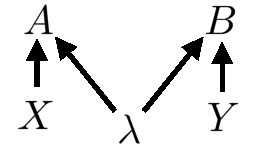
\includegraphics[width=3cm]{Bell.pdf}}
\caption{The causal structure on which Bell's theorem is based.}
 \label{fig:Bell}
\end{figure}


The outcome and setting on the left are labelled $A$ and $X$, the outcome and the setting on the right are labelled $B$ and $Y$, while the common cause hidden variable is labelled $\lambda$.  Note, that we will deviate from the notation used in the quote given above by denoting the two settings by $X\in \{ 0,1\}$ rather than $X\in \{ 1,2\}$.

One can cast the Hardy proof as follows:
\begin{proposition} \label{prop:Hardy}
For the causal structure of Fig.~\ref{fig:Bell}, the following inference holds
\begin{align}
{\rm if  }\;\; p(A=1,B=1|X=0,Y=0)>0  \label{ass1}\\
{\rm and }\;\; p(B=1|Y=1,A=1,X=0) =1 \label{ass2}\\
{\rm and }\;\; p(A=1|X=1,B=1,Y=0) =1 \label{ass3}\\
{\rm then }\;\; p(A=1,B=1|X=1,Y=1)>0. \label{ass4}
\end{align}
\end{proposition}

As Hardy has shown, there exist quantum correlations that violate this inference (i.e. satisfy the antecedents, \eqref{ass1}-\eqref{ass3} but violate the consequent \eqref{ass4}).  It follows that these quantum correlations cannot 
%It follows that any observed distribution that violates this inference, such as occurs with the quantum correlations described by Hardy, cannot 
be explained by the causal structure of Fig.~\ref{fig:Bell}.


\begin{proof}
From the causal structure, we can infer that the LHS of Eq.~\eqref{ass2} can be expressed as
\begin{equation}
p(B=1|Y=1,A=1,X=0) = \sum_{\lambda} p(B=1|Y=1,\lambda) p(\lambda|A=1, X=0).
\end{equation}
From Eq.~\eqref{ass2} it follows that
\begin{equation}\label{star1}
\forall \lambda:
%\; \textrm{such that}\; 
p(\lambda|A=1,X=0)>0, \textrm{ we have}\; p(B=1|Y=1,\lambda)=1.
\end{equation}

Similarly, from the causal structure, we can infer that the LHS of Eq.~\eqref{ass3} can be expressed as
\begin{equation}
p(A=1|X=1,B=1,Y=0) = \sum_{\lambda} p(A=1|X=1,\lambda) p(\lambda|B=1, Y=0).
\end{equation}
and from Eq.~\eqref{ass3} it then follows that
\begin{equation}\label{star2}
\forall \lambda:
%\; \textrm{such that}\; 
p(\lambda|B=1,Y=0)>0, \textrm{ we have}\; p(A=1|X=1,\lambda)=1.
\end{equation}

Finally, from the causal structure, we can infer that the LHS of Eq.~\eqref{ass1} can be expressed as
\begin{equation}
p(A=1,B=1|X=0,Y=0) = \sum_{\lambda} p(A=1|X=0,\lambda) p(\lambda|B=1|Y=0,\lambda)p(\lambda).
\end{equation}
It then follows from  Eq.~\eqref{ass1}  that there must exist a value of $\lambda$, which we denote $\lambda_*$ such that
\begin{align}
p(\lambda_*)&>0,\label{ineq1}\\
p(A=1|X=0,\lambda_*)&>0,\\
p(B=1|Y=0,\lambda_*)&>0.
\end{align}
By Bayesian inversion, we obtain
\begin{align}
p(\lambda_*|A=1,X=0)=\frac{p(A=1|X=0,\lambda_*)p(\lambda_*)}{p(A=1)}&>0,\\
p(\lambda_*|B=1,Y=0)=\frac{p(B=1|Y=0,\lambda_*)p(\lambda_*)}{p(B=1)}&>0.
\end{align}

It then follows from Eqs~\eqref{star1} and \eqref{star2} that
\begin{align}
p(B=1|Y=1,\lambda_*)=1 \label{det1}\\
p(A=1|X=1,\lambda_*)=1. \label{det2}
\end{align}

Finally, from the causal structure, we can infer that the LHS of Eq.~\eqref{ass4} can be expressed as
\begin{equation}\label{final}
p(A=1,B=1|X=1,Y=1)= \sum_{\lambda} p(A=1|X=1,\lambda) p(B=1|Y=1,\lambda) p(\lambda).
\end{equation}
Making use of Eqs.~\eqref{ineq1}, \eqref{det1} and \eqref{det2}, we obtain Eq.~\eqref{ass4}.
\end{proof}


\clearpage
\section{The triangle causal structure (original)}

We now consider the causal structure depicted in Fig.~\ref{fig:triangle}.

\begin{figure}[h!]
 \center{   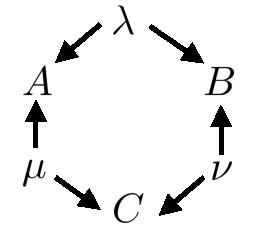
\includegraphics[width=3cm]{triangle.pdf}}
\caption{The triangle causal structure. }
 \label{fig:triangle}
\end{figure}

The three observed variables are denoted $A$, $B$ and $C$, while $\lambda$ denotes the common cause of $A$ and $B$, $\mu$ denotes the common cause of $A$ and $C$, and $\nu$ denotes the common cause of $B$ and $C$.

\begin{proposition}\label{prop:triangle}
The causal structure of Fig.~\ref{fig:triangle} implies the following inference
\begin{align}
{\rm if } \;\; p(A=1)>0\\
{\rm and}\;\; p(B=1)>0\\
{\rm and} \;\; p(C=1)>0 \\
{\rm and }\;\; A=1 \implies B=0  \\
%{\rm and }\;\; A=1 \implies C=0 \\
%{\rm and  }\;\; B=1 \implies A=0  \\
{\rm and }\;\; B=1 \implies C=0 \\
{\rm and  }\;\; C=1 \implies A=0  \\
%{\rm and }\;\; C=1 \implies B=0\\
{\rm then }\;\; p(A=0,B=0,C=0)>0. 
\end{align}
\end{proposition}

We can express this in terms of conditional probabilities as follows
%The triangle causal structure implies the following inference
\begin{align}
{\rm if } \;\; p(A=1)>0 \label{s1}\\
{\rm and}\;\; p(B=1)>0 \label{s2}\\
{\rm and} \;\; p(C=1)>0 \label{s3}\\
{\rm and}\;\; p(B=0|A=1)=1  \label{t1}\\
%{\rm and }\;\; p(C=0|A=1) =1 \label{t2}\\
%{\rm and  }\;\; p(A=0|B=1)=1  \label{t3}\\
{\rm and }\;\; p(C=0|B=1) =1 \label{t4}\\
%{\rm and }\;\; p(B=0|C=1) =1 \label{t5}\\
{\rm and  }\;\; p(A=0|C=1)=1  \label{t6}\\
{\rm then }\;\; p(A=0,B=0,C=0)>0. \label{t7}
\end{align}

Given the inference, one can show that the distribution
\begin{equation}\label{eq:wdistribution}
p(A,B,C) = \frac{1}{3} \left( [001] + [010] + [100]\right).
\end{equation}
is inconsistent with the triangle causal structure.   The reason is that this distribution satisfies the antecedent of the inference, Eqs.~\eqref{s1}-\eqref{s3} and Eqs.~\eqref{t1}-\eqref{t6}, and yet it violates the consequent of the inference, Eq.~\eqref{t7}.

It is an open question whether this distribution can be realized quantum mechanically or in a generalized probabilistic theory.

\begin{proof}
Given the causal structure, the LHS of Eq.~\eqref{t1} can be expressed as
\begin{equation}
p(B=0|A=1) = \sum_{\lambda,\nu} p(B=0|\lambda,\nu) p(\lambda|A=1) p(\nu).
\end{equation} 
Then from Eq.~\eqref{t1}, it follows that 
\begin{equation}\label{star1b}
\forall \nu \forall \lambda: p(\nu)>0,\; p(\lambda|A=1)>0,\; \textrm{ we have}\; p(B=0|\lambda,\nu)=1.
\end{equation}

Using this same pattern of argument for each of the three inferences \eqref{t1}-\eqref{t6}, we get the following three results:
\begin{align}
&\forall \nu \forall \lambda: p(\nu)>0,\; p(\lambda|A=1)>0,\; \textrm{ we have}\; p(B=0|\lambda,\nu)=1, \label{c1} \\
%&\forall \mu \forall \nu: p(\nu)>0,\; p(\mu |A=1)>0,\; \textrm{ we have}\; p(C=0|\mu,\nu)=1, \\
&\forall \mu \forall \nu: p(\mu)>0,\; p(\nu|B=1)>0,\; \textrm{ we have}\; p(C=0|\nu,\mu)=1, \\
%&\forall \mu \forall \lambda: p(\mu)>0,\; p(\lambda |B=1)>0,\; \textrm{ we have}\; p(A=0|\lambda,\mu)=1, \\
&\forall \lambda \forall \mu: p(\lambda)>0,\; p(\mu|C=1)>0,\; \textrm{ we have}\; p(A=0|\lambda,\mu)=1, \\
%&\forall \nu \forall \lambda: p(\lambda)>0,\; p(\nu |C=1)>0,\; \textrm{ we have}\; p(B=0|\nu,\lambda)=1, 
\end{align}

Given the causal structure, we can express $p(A=1)$ as
\begin{equation}
p(A=1)= \sum_{\lambda,\mu} p(A=1|\lambda, \mu)\; p(\lambda,\mu).
\end{equation}
Combining this with the fact that $p(A=1)>0$, Eq.~\eqref{s1}, it follows that there exist values of $\lambda$ and $\mu$, which we denote $\lambda_*$ and $\mu_0$, such that 
\begin{align}
p(\lambda_*,\mu_0)>0\\
p(A=1| \lambda_*, \mu_0)>0.
\end{align}
From the causal structure, we infer that 
\begin{align}
p(\lambda_*,\mu_0)= p(\lambda_*)p(\mu_0),
\end{align}
so that we have 
\begin{align}
p(\lambda_*)>0\\
p(\mu_0)>0.
\end{align}
It also follows from the causal structure that 
\begin{align}
p(A=1| \lambda_*) = \sum_{\mu} p(A=1| \lambda_*, \mu) p(\mu),
\end{align}
and consequently
\begin{align}
p(A=1| \lambda_*) >0.
\end{align}
By Bayesian inversion, we have
\begin{align}
p(\lambda_*|A=1)= \frac{p(A=1| \lambda_*) p(\lambda_*)}{p(A=1)} >0.
\end{align}
Finally, recalling Eq.~\eqref{c1}, we can infer that 
%there exists a $\lambda_*$ such that
%\begin{align}
%&p(\lambda_*) > 0, \nonumber\\
%&\forall \nu : p(\nu)>0\;  \textrm{ we have}\; p(B=0|\lambda_*,\nu)=1. \label{x1}
%\end{align}
%Altogether then, we have shown that  
there exists a $\lambda_*$ such that
\begin{align}
&p(\lambda_*) > 0, \nonumber\\
&\forall \nu : p(\nu)>0\;  \textrm{ we have}\; p(B=0|\lambda_*,\nu)=1. \label{x1}
\end{align}


By similar arguments, we can derive that there exists a $\mu_*$ such that
\begin{align}
&p(\mu_*) > 0, \nonumber\\
&\forall \lambda : p(\lambda)>0\;  \textrm{ we have}\; p(C=0|\lambda,\mu_*)=1. \label{x2}
\end{align}
and there exists a $\nu_*$ such that
\begin{align}
&p(\nu_*) > 0, \nonumber\\
&\forall \mu : p(\mu)>0\;  \textrm{ we have}\; p(A=0|\mu,\nu_*)=1.  \label{x3}
\end{align}

Finally, given the causal structure, we can express the LHS of Eq.~\eqref{t7} as
\begin{equation}
p(A=0,B=0,C=0)= \sum_{\lambda, \mu,\nu} p(A=0|\lambda,\mu) p(B=0|\lambda,\nu) p(C=0|\mu,\nu) p(\lambda)p(\mu)p(\nu).
\end{equation}
In particular, this implies that
\begin{align}
p(A=0,B=0,C=0) &\ge p(A=0|\lambda_*,\mu_*) p(B=0|\lambda_*,\nu_*) p(C=0|\mu_*,\nu_*) p(\lambda_*)p(\mu_*)p(\nu_*). \nonumber
\end{align}

It then follows from Eqs.~\eqref{x1}, \eqref{x2} and \eqref{x3} that
\begin{align}
p(A=0,B=0,C=0) 
%&\ge p(A=0|\lambda_*,\mu_*) p(B=0|\lambda_*,\nu_*) p(C=0|\mu_*,\nu_*) p(\lambda_*)p(\mu_*)p(\nu_*) \nonumber\\
&\ge p(\lambda_*)p(\mu_*)p(\nu_*)\nonumber\\
&> 0
\end{align}
Therefore, we have proven Eq.~\eqref{t7}.
\end{proof}







%Let the common cause of $A$ and $B$ be denoted $\lambda$, of $A$ and $C$ be denoted $\mu$, and of $B$ and $C$ be denoted $\nu$.

\purp{
\section{Hardy-type inferences can be stronger than all Entropic Inequalities}
In Causal Inference there is a well-established technique for deriving entropic inequalities implied by a given causal structure \cite{fritz2013marginal,chaves2014novel}. For the causal structure associated with Bell's theorem in Fig.~\ref{fig:Bell}, for example, there is a well known entropic Bell inequality \cite{chaves2014novel,chaves2012entropic}. Like its corresponding probabilistic Bell inequality, the entropic variant is is capable of excluding many distributions which one could not exclude by considering only conditional independence relations. Indeed, the enumeration of all entropic inequalities which follow from a given causal structure is currently the state-of-the-art method for capturing implications from the causal structure beyond conditional independence relations \cite{pusey2014gdag}.

However, the method of entropic inequalities is not completely sufficient. For at least some causal structures, there are disallowed probability distributions which manage to evade detection when tested against the complete set of entropic inequalities. Of course, if a distribution passes all the entropic inequalities, it usually takes some ingenuity to prove that it is nevertheless incompatible with the causal structure. The triangle scenario of Fig.~\ref{fig:triangle} is a causal structure who's complete set of entropic inequalities is known to be insufficient \cite{fritz2012bell}. However, the question of the sufficiency of the complete set of entropic inequalities was not answered for the case where the three observed variables in the triangle are binary.  We answer it here in the negative by showing that the distibution in Eq.~\eqref{eq:wdistribution} satisfies all entropic inequalities, but is nevertheless disallowed perusant to the Hardy-type inference of \textbf{Prop.~\ref{prop:triangle}}.

In the triangle scenario there are precisely three unique fundamental entropic inequalities, under the obvious symmetry of relabelling the three observed variables. They are
\begin{align}
H\!\left(A\right)&\geq I\!\left(A:B\right)+I\!\left(A:C\right)\label{eq:entropicineq1} \\
H\!\left(A,B\right)&\geq I\!\left(A:B:C\right)+I\!\left(A:B\right)+I\!\left(A:C\right)+I\!\left(B:C\right)\label{eq:entropicineq2}\\
\frac{H\!\left(A\right)+H\!\left(B\right)+H\!\left(C\right)}{2} &\geq I\!\left(A:B:C\right)+I\!\left(A:B\right)+I\!\left(A:C\right)+I\!\left(B:C\right)\label{eq:entropicineq3}
\end{align}
where bipartite mutual information may be understood as $I\!\left(A:B\right)\equiv H\!\left(A\right)+H\!\left(B\right)-H\!\left(A,B\right)$ and tripartite mutual information is defined as $I\!\left(A:B:C\right)\equiv H\!\left(A\right)+H\!\left(B\right)+H\!\left(C\right)-H\!\left(A,B\right)-H\!\left(A,C\right)-H\!\left(B,C\right)+H\!\left(A,B,C\right)$.
An entropy is a weighted logarithmic sum of probabilities, for binary variables 
\begin{align}\begin{split}
H\!\left(A,B,C\right)&=\sum\limits_{a,b,c=0}^1
\begin{cases} p\!\left(A=a,B=a,C=c\right)\log\left(\frac{1}{p\left(A=a,B=a,C=c\right)}\right) & p\!\left(A=a,B=a,C=c\right) > 0 \\ 0 & p\!\left(A=a,B=a,C=c\right)=0 \end{cases} \\
H\!\left(A,B\right)&=\sum\limits_{a,b=0}^1
\begin{cases} p\!\left(A=a,B=a\right)\log\left(\frac{1}{p\left(A=a,B=a\right)}\right) & p\!\left(A=a,B=a\right) > 0 \\ 0 & p\!\left(A=a,B=a\right)=0 \end{cases} \\
H\!\left(A\right)&=\sum\limits_{a=0}^1
\begin{cases} p\!\left(A=a\right)\log\left(\frac{1}{p\left(A=a\right)}\right) & p\!\left(A=a\right) > 0 \\ 0 & p\!\left(A=a\right)=0 \end{cases}\,.
\end{split}\end{align}
The base of the logarithm is conventionally taken to be 2, but the base is irrelevant for the purpose of evaluating entropic inequalities. Applied to the symmetric distribution of Eq.~\eqref{eq:wdistribution} we find
\begin{align}
H\!\left(A,B,C\right)=H\!\left(A,B\right)=\log\left(3\right)\text{ and }H\!\left(A\right)=\log\left(3\times 2^{-\nicefrac{2}{3}}\right)
\end{align}

From these definitions it is straightforward to verify that the W-type distribution of Eq.~\eqref{eq:wdistribution} respects Eqs.~\eqref{eq:entropicineq1}-\eqref{eq:entropicineq3}, thus illustrating the advantage of Hardy-type inference over entropic inequalities in terms of recognizing this distribution as incompatible with the triangle scenario.
}

\section{From inferences concerning observed variables to inequalities}

I suspect that using the same techniques that Ravi Kunjwal and I have used for deriving noncontextuality inequalities, we can replace the inference in proposition \ref{prop:Hardy} with an inequality.  Perhaps something like
\begin{align}
&p(A=1,B=1|X=1,Y=1) \nonumber \\
&\ge p(B=1| Y=1,A=1,X=0)\; p(A=1| X=1,B=1,Y=0) \; p(A=1,B=1|X=0,Y=0).
\end{align}
I will need to think about this more.  

A different approach would be to look to the pre-existing literature that seeks to derive Bell inequalities from Hardy-type reasoning.  It appears that many groups have considered this question~\cite{Mermin2,Garuccio95,Ghirardi08,Braun08,Mancinska14} (it is unclear whether this list of references is complete).

The idea is that perhaps one of these approaches can be generalized such that we can derive inequalities for the triangle causal structure.
%If this works, then one can presumably derive inequalities for the triangle causal structure in a similar fashion.


I will may a small start on this problem here by considering the approach of Ghirardi and Marinotta.  They state that: ``we have shown that the existing Hardy-like nonlocality without inequalities proofsfor bipartite states [...] are simply particular instances of violations of the Clauser-Horne inequality.''  If we believe their claim, then it implies that turning the Hardy-type reasoning about transitivity of inferences into an inequality results in precisely the CH inequality, which we can summarize as follows.
\begin{proposition} %\label{prop:Hardy}
For the Bell-scenario causal structure of Fig.~\ref{fig:Bell}, the following inequality holds
\begin{align}
0 \le &p(A=1,B=1|X=0,Y=0) \nonumber\\
&-p( A=1,B=1 |X=0,Y=1)\nonumber\\
&-p(A=1, B=1|X=1,Y=0)\nonumber\\
&-p(A=1,B=1|X=1,Y=1)\nonumber\\
& + p(A=1|X=1) + p(B=1|Y=1) \le 1.
\end{align}
\end{proposition}

Their argument relies on looking at the measures of various sets.  Inspired by the details of their proof, can we use similar reasoning in the context of the triangle causal structure to get some inequalities?

The Ghirardi and Marinotta argument looks similar to the way that Tobias describes how he derived some inequalities for the triangle causal structure.  I suspect, therefore, that this approach might just lead to the inequalities that Tobias has already found.  Even if it did, it would be interesting to draw the parallel with the Hardy paradox situation.

It might be worth looking at some of the other papers in the list I provided to see if the reasoning there can be ported over to the triangle causal structure. 
\end{comment}

\begin{acknowledgments}
Research at Perimeter Institute is supported by the Government of Canada through Industry Canada and by the Province of Ontario through the Ministry of Economic Development and Innovation.
\end{acknowledgments}

%\section*{References}
\nocite{*}
%\setlength{\bibsep}{\smallskipamount}
\bibliographystyle{apsrev4-1}
%nocite{apsrev41Control}
\bibliography{apsrevcontrol,hardyinference}

%\begin{references}

%\bibitem{WoodSpekkens} C. J. Wood and R. W. Spekkens, ``The lesson of causal discovery algorithms for quantum correlations: Causal explanations of Bell-inequality violations require fine-tuning'', arXiv:1208.4119 (quant-ph).

%\bibitem{LSW} Y.\ C.\ Liang, R.\ W.\ Spekkens, H.\ M.\ Wiseman, ``Specker's parable of the overprotective seer: A road to contextuality, nonlocality and complementarity''. Phys. Rep. {\bf 506}, 1 (2011).

%\bibitem{L.Hardy:PRL:1665} L.~Hardy, \prl {\bf 71}, 1665 (1993).

%\bibitem{D.Boschi:PRL:2755} D.~Boschi, S.~Branca, F.~De~Martini, and L.~Hardy, \prl {\bf 79}, 2755 (1997).
    
%\bibitem{H.Stapp:Hardy:Transitivity} H.~P.~Stapp, {\em Mind, Matter, and Quantum Mechanics} (Springer-Verlag, Berlin, 1993); Am.~J.~Phys. {\bf 65}, 300 (1997).

%\bibitem{Mermin} N.~D.~Mermin, arXiv:quant-ph/9711052v1.

%\bibitem{Unruh} W. Unruh, arXiv:quant-ph/9710032v2.

%\bibitem{Mermin2} N. David Mermin. Quantum mysteries refined. Am. J. Phys., 62(10):880�886, 1994.doi:10.1119/1.17733.

%\bibitem{Garuccio95} Augusto Garuccio. Hardy�s approach, Eberhard�s inequality, and supplementary assumptions.Phys. Rev. A, 52:2535�2537, 1995. doi:10.1103/PhysRevA.52.2535.

%\bibitem{Ghirardi08} GianCarlo Ghirardi and Luca Marinatto. Proofs of nonlocality without inequalitiesrevisited. Phys. Lett. A, 372(12):1982�1985, 2008. arXiv:0711.0505, doi:10.1016/j.physleta.2007.11.012.

%\bibitem{Braun08} Daniel Braun and Mahn-Soo Choi. Hardy�s test versus the Clauser-Horne-Shimony-Holt test of quantum nonlocality: Fundamental and practical aspects. Phys. Rev. A,78(3):032114, 2008. arXiv:0808.0052, doi:10.1103/PhysRevA.78.032114.

%\bibitem{Mancinska14} Laura Mancinska and Stephanie Wehner, A unified view on Hardy's paradox and the CHSH inequality, arXiv:1407.2320.

%\end{references}

\end{document}